 \documentclass[xcolor=dvipsnames,table]{beamer}

\usepackage{latexsym}
\usepackage[utf8]{inputenc}
\usepackage[brazil]{babel}
\usepackage{amssymb}
\usepackage{amsmath}
\usepackage{stmaryrd}
\usepackage{fancybox}
\usepackage{datetime}
\usepackage[T1]{fontenc}
\usepackage{graphicx}
\usepackage{graphics}
\usepackage{url}
\usepackage{algorithmic}
\usepackage{algorithm}
\usepackage{acronym}
\usepackage{array}

\usepackage{enumitem}

\newtheorem{definicao}{Definio}
\newcommand{\tab}{\hspace*{2em}}

\mode<presentation>
{
  \definecolor{colortexto}{RGB}{0,0,0}
 
  \setbeamertemplate{background canvas}[vertical shading][ bottom=white!10,top=white!10]
  \setbeamercolor{normal text}{fg=colortexto} 

  \usetheme{Warsaw}
}

\title[Inteligência Artificial e Trabalho Docente]{Inteligência Artificial e Trabalho Docente\\
{\small Diferentes concepções de inteligência e seus impactos na docência}
}  

\author{
  Esdras Lins Bispo Jr. \\ \url{bispojr@ufj.edu.br}
  } 
 \institute{
  Mestrado Profissional em Educação em Computação (ProfComp) \\Bacharelado em Ciência da Computação (BCC)\\
  Universidade Federal de Jataí (UFJ)}
\date{\textbf{16 de março de 2026} }

\logo{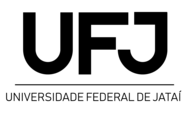
\includegraphics[width=1.5cm]{images/ufjJataiLogo.png}}

\begin{document}

	\begin{frame}
		\titlepage
	\end{frame}

	\AtBeginSubsection[]{
    \begin{frame}{Sumário}%[allowframebreaks]{Sumário}
        \tableofcontents[currentsection, currentsubsection]
    \end{frame}
}

	\begin{frame}{Plano de Aula}
		\tableofcontents
		
	\end{frame}
	
\section{Introdução}

\begin{frame}{Introdução}
    \begin{block}{Lentes para olhar a Educação}
        \begin{itemize}[label=\textbullet]
            \item Definição de Inteligência Artificial $\rightarrow$ \\Concepção sobre Tecnologia educacional;
            \item Conceito de Inteligência $\rightarrow$ Conceito de Aprendizagem;
            \item (e consequentemente uma forma diferente \\de imaginar o papel do professor).
        \end{itemize}
        
    \end{block}
    
\end{frame}
    
\section{Linhas mais Clássicas}
\subsection{Agir de forma humana}

   \begin{frame}{Agir de forma humana}
        \begin{block}{}
            Pensar {\it vs} \underline{Agir} \ \ \underline{Forma humana} {\it vs} Forma racional
        \end{block}
        
		\begin{center}
            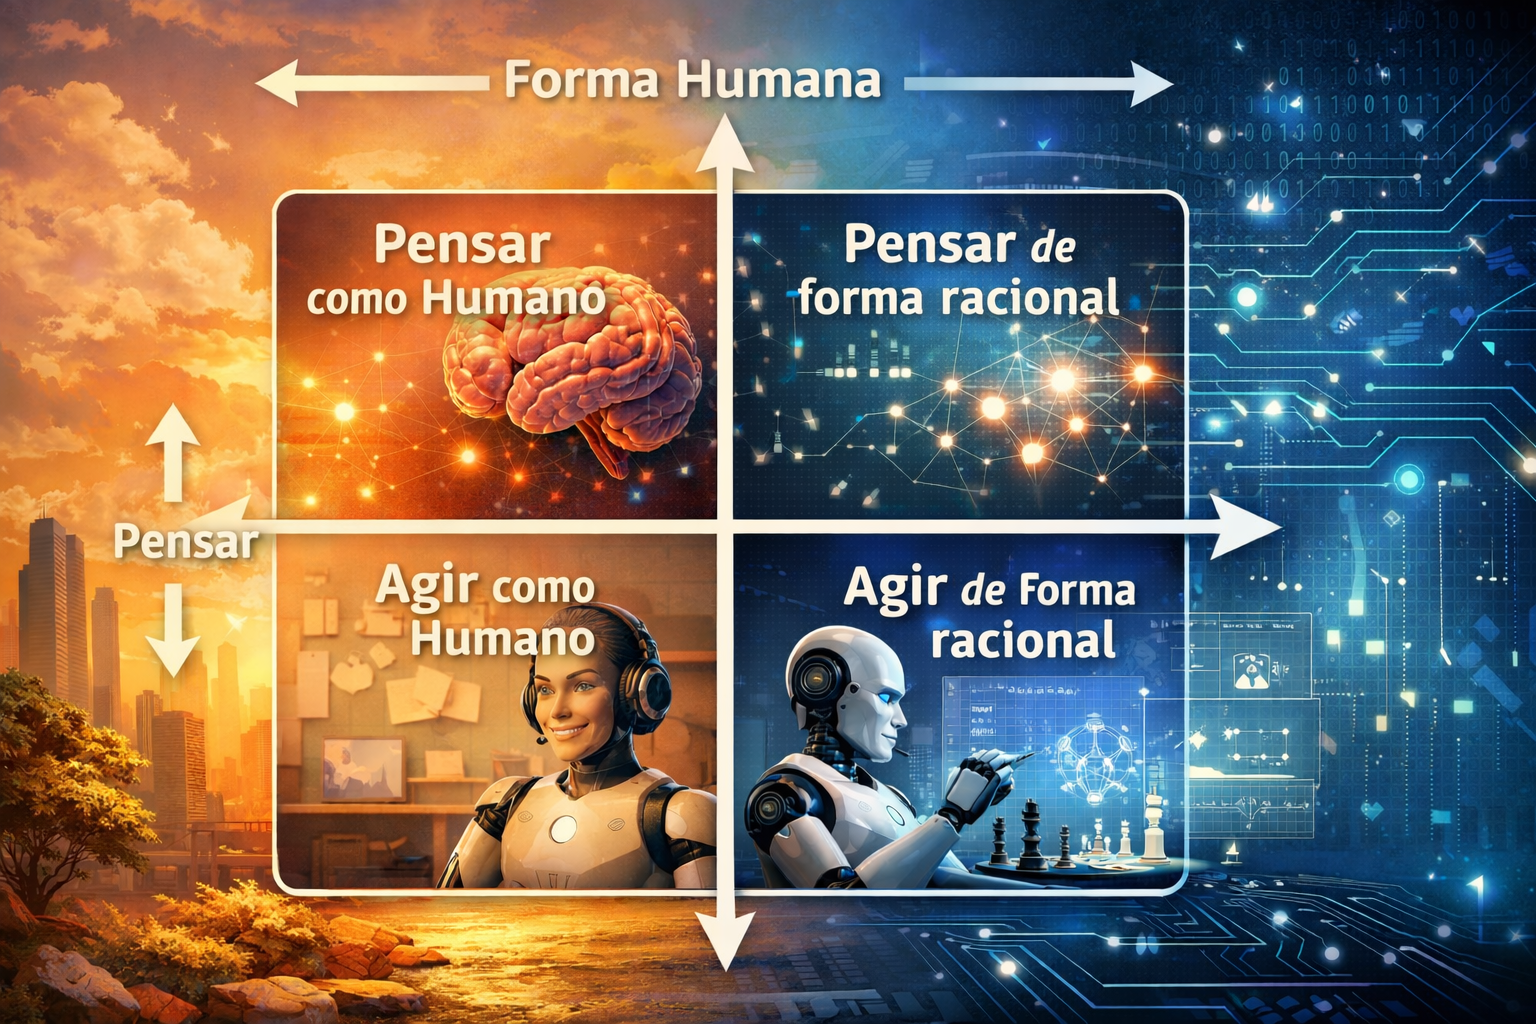
\includegraphics
            [width=0.8\textwidth]{images/pensar-forma.png}
        \end{center}
        
	\end{frame}  

    \begin{frame}{Agir de forma humana}
        \begin{block}{Ideia Geral}
            Essa linha tenta {\bf imitar comportamento humano}.        
        \end{block} \pause
		\begin{block}{Kurweil, 1990}
			``A arte de criar máquinas que executam funções que exigem inteligência quando executadas por pessoas''
		\end{block} \pause
		\begin{exampleblock}{Exemplo}
			Teste de Turing
		\end{exampleblock}
	\end{frame}

    \begin{frame}{Teste de Turing}
        
        \begin{center}
            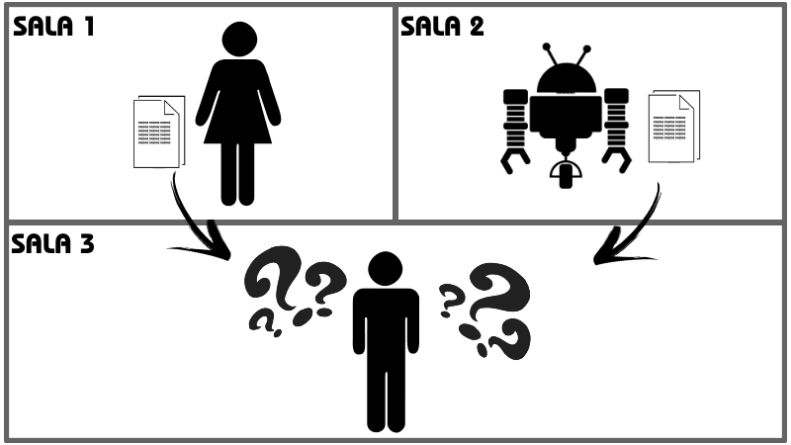
\includegraphics
                [width=\textwidth]{images/teste-turing.png}
        \end{center}
        
    \end{frame}

    \begin{frame}{Agir de forma humana}
        \begin{block}{Ideia Geral}
            Essa linha tenta {\bf imitar comportamento humano}.        
        \end{block} 
		\begin{block}{Kurweil, 1990}
			``A arte de criar máquinas que executam funções que exigem inteligência quando executadas por pessoas''
		\end{block} 
		\begin{exampleblock}{Provocações para a pesquisa em Educação}
			Se um aluno aprende conversando com uma IA, \\isso é diferente de aprender com um humano?
		\end{exampleblock}
	\end{frame}

\subsection{Pensar de forma humana}
    
    \begin{frame}{Pensar de forma humana}
        \begin{block}{}
            \underline{Pensar} {\it vs} Agir \ \ \underline{Forma humana} {\it vs} Forma racional
        \end{block}
        
		\begin{center}
            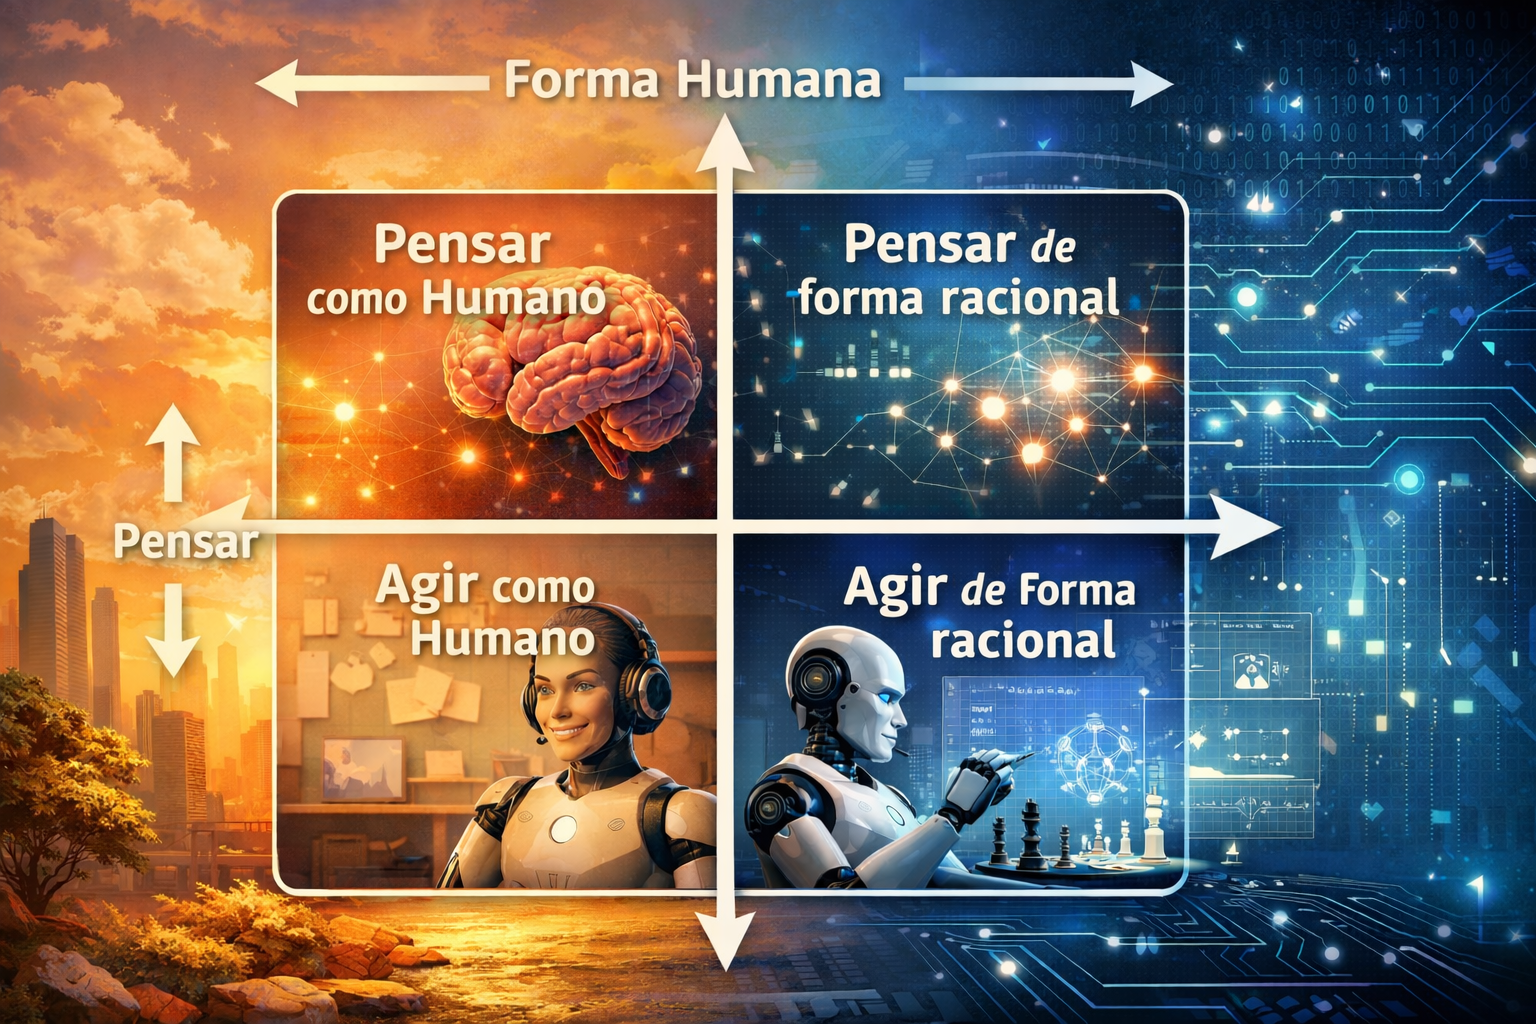
\includegraphics
            [width=0.8\textwidth]{images/pensar-forma.png}
        \end{center}
        
	\end{frame} 

    \begin{frame}{Pensar de forma humana}
        \begin{block}{Ideia Geral}
            Essa linha tenta {\bf simular os processos mentais humanos}.        
        \end{block} \pause
		\begin{block}{Charniak e McDermott, 1985}
			``O estudo das faculdades mentais \\pelo uso de modelos computacionais''
		\end{block}\pause
		\begin{exampleblock}{Exemplo}
			Modelagem cognitiva
		\end{exampleblock}
	\end{frame}

    \begin{frame}{Modelagem Cognitiva}
        
        \begin{center}
            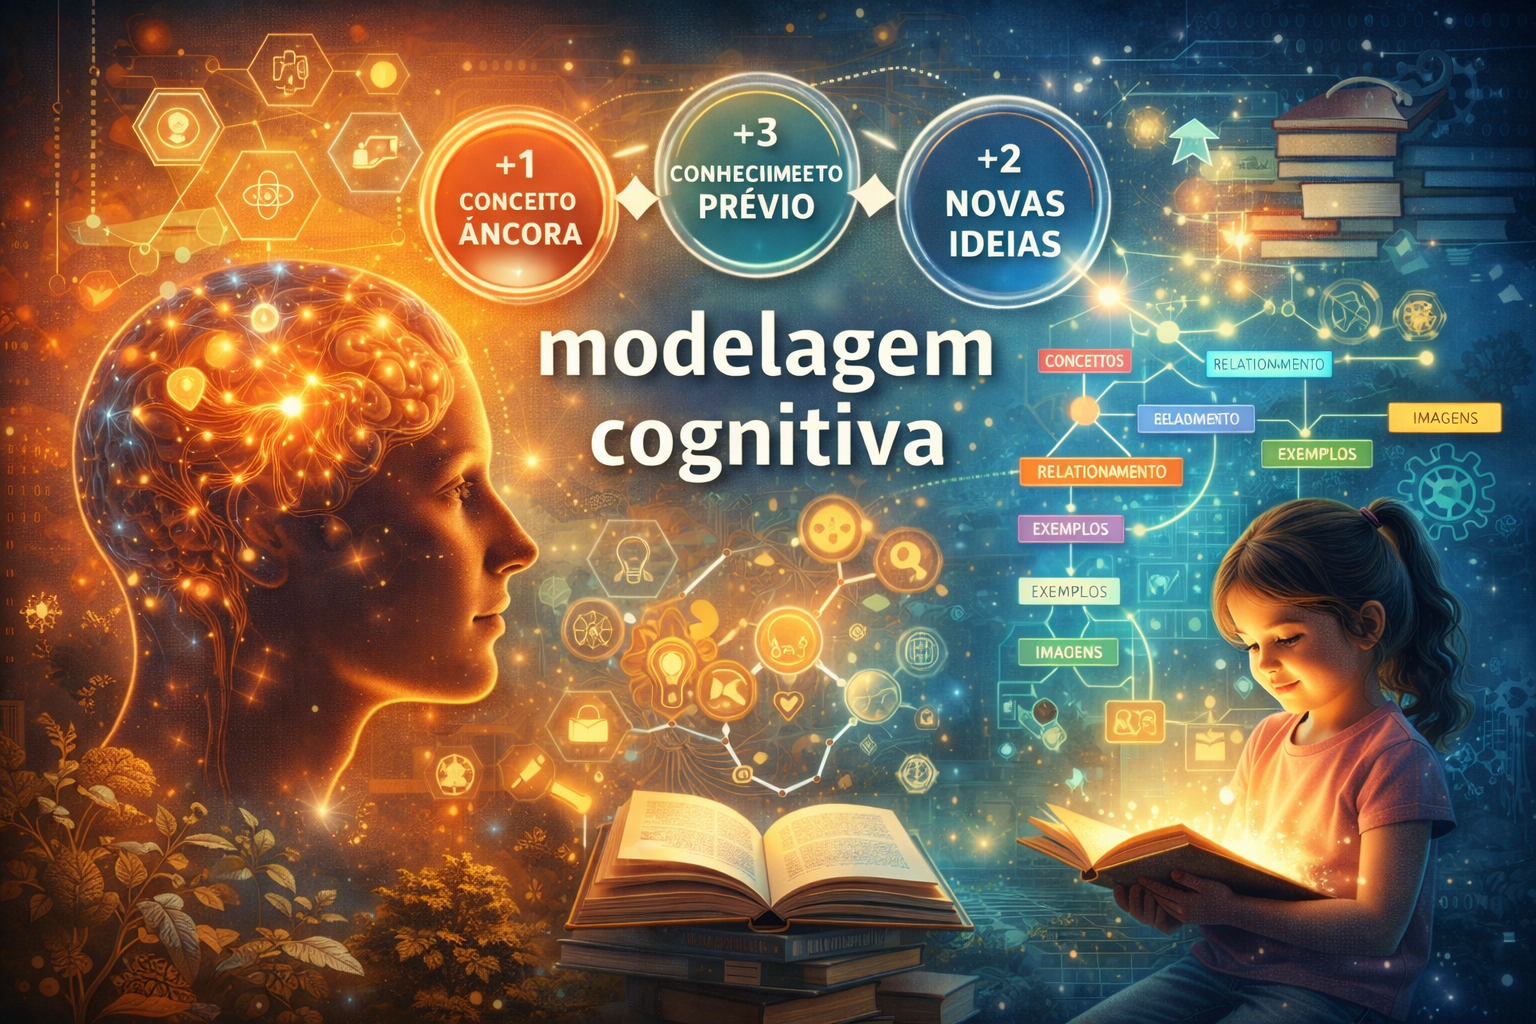
\includegraphics
                [width=\textwidth]{images/modelagem-cognitiva.png}
        \end{center}
        
    \end{frame}

    \begin{frame}{Pensar de forma humana}
        \begin{block}{Ideia Geral}
            Essa linha tenta {\bf simular os processos mentais humanos}.        
        \end{block}
		\begin{block}{Charniak e McDermott, 1985}
			``O estudo das faculdades mentais \\pelo uso de modelos computacionais''
		\end{block}
		\begin{exampleblock}{Provocação para a Pesquisa em Educação}
			Um sistema tenta identificar qual estado mental \\o aluno está ao resolver um problema.
            \begin{itemize}[label=\textbullet]
                \item A IA pode inferir o raciocínio do aluno?
                \item Isso muda a forma de avaliação?
            \end{itemize}
		\end{exampleblock}
	\end{frame}    

\subsection{Pensar de forma racional}
    
    \begin{frame}{Pensar de forma racional}
        \begin{block}{}
            \underline{Pensar} {\it vs} Agir \ \ Forma humana {\it vs} \underline{Forma racional}
        \end{block}
        
		\begin{center}
            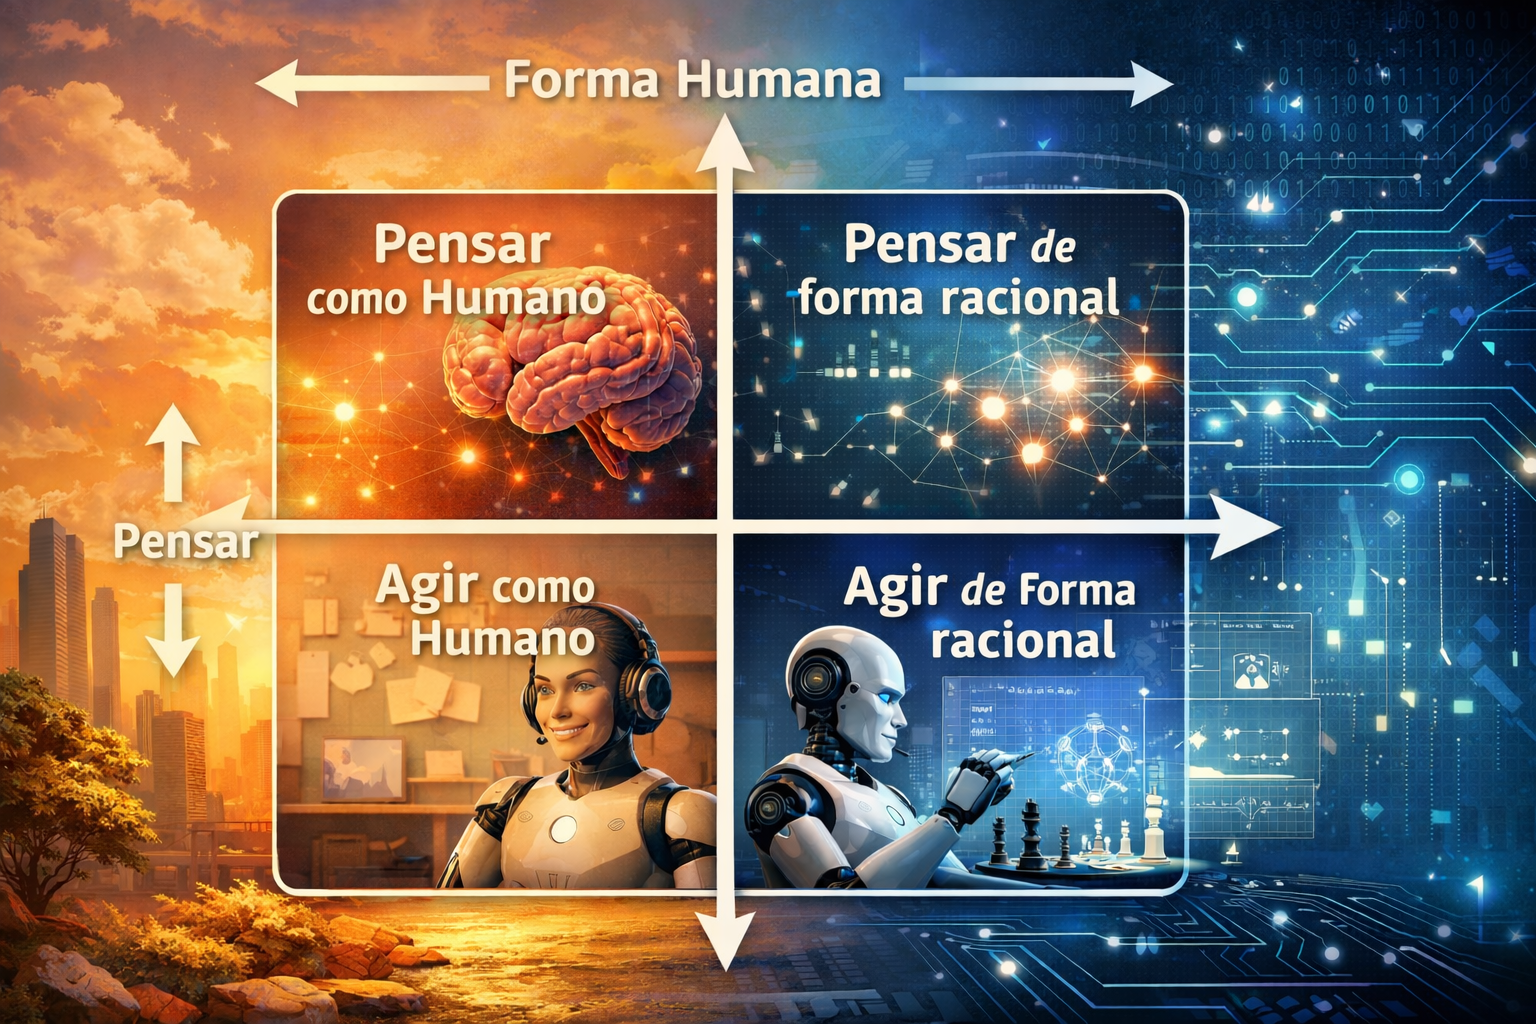
\includegraphics
            [width=0.8\textwidth]{images/pensar-forma.png}
        \end{center}
        
	\end{frame} 

    \begin{frame}{Pensar de forma racional}
        \begin{block}{Ideia Geral}
            Essa linha tenta {\bf representar o conhecimento de forma lógica e produzir inferências válidas}.        
        \end{block} \pause
		\begin{block}{McCarthy e Hayes, 1969}
			``O estudo da representação do conhecimento \\e os mecanismos para o raciocínio sobre aquele conhecimento''.
		\end{block}\pause
		\begin{exampleblock}{Exemplo}
			Raciocínio correto por meio de lógica formal.
		\end{exampleblock}
	\end{frame}

    \begin{frame}{Representação do Conhecimento}
        
        \begin{center}
            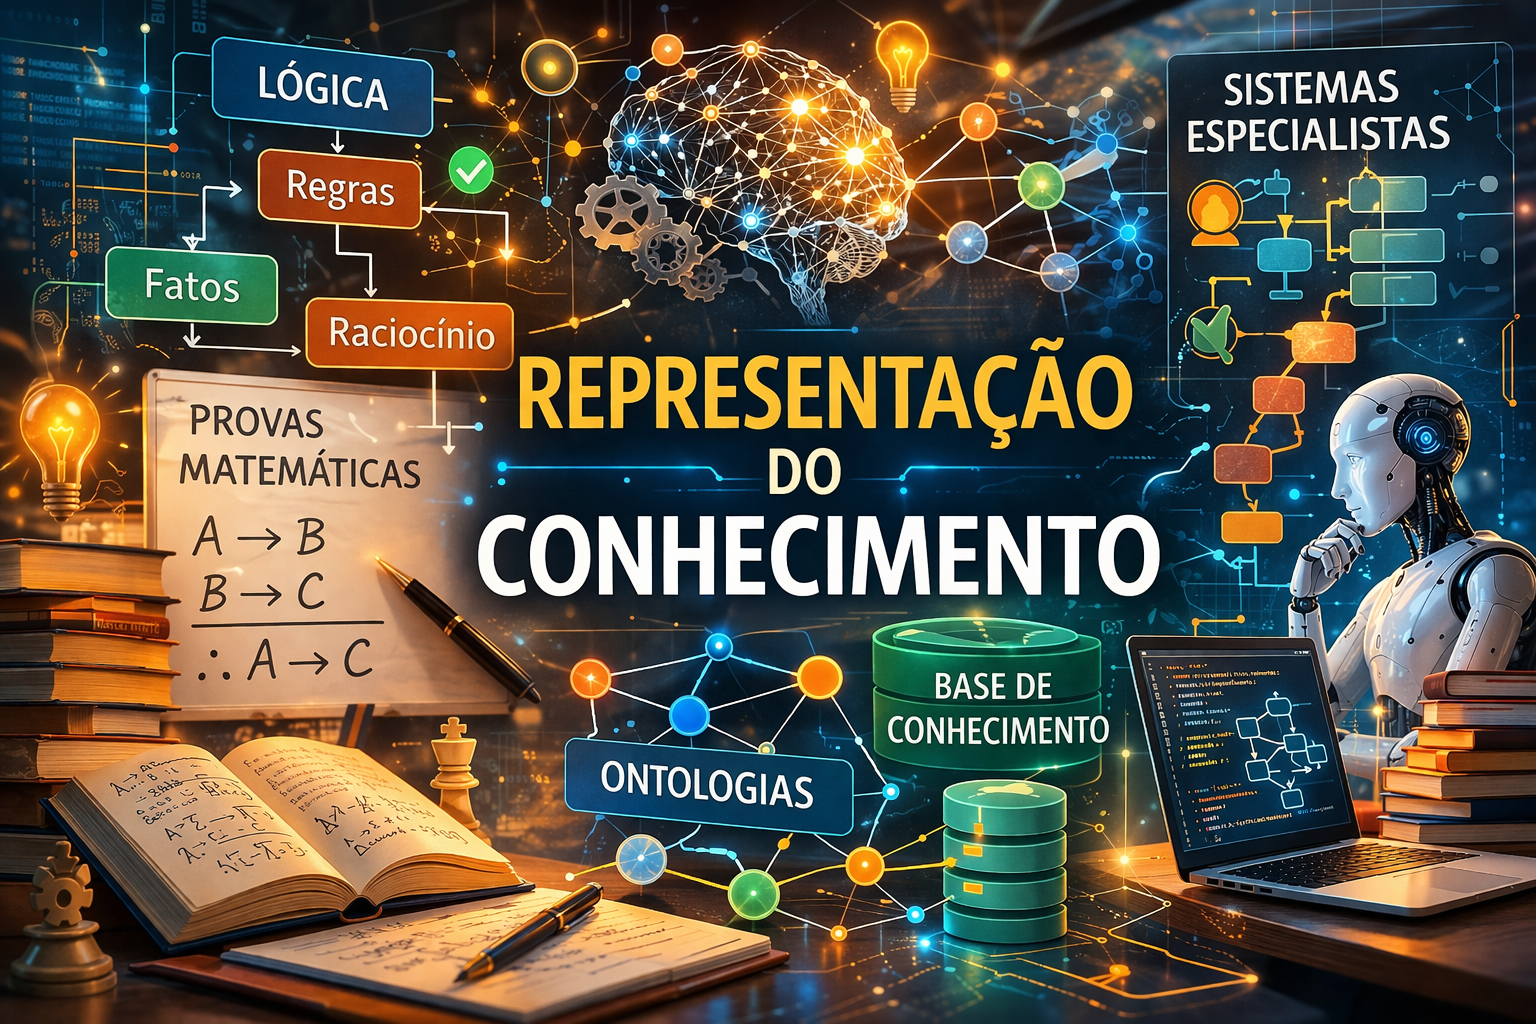
\includegraphics
                [width=\textwidth]{images/representacao-conhecimento.png}
        \end{center}
        
    \end{frame}

    \begin{frame}{Pensar de forma racional}
        \begin{block}{Ideia Geral}
            Essa linha tenta {\bf representar o conhecimento de forma lógica e produzir inferências válidas}.        
        \end{block}
		\begin{block}{McCarthy e Hayes, 1969}
			``O estudo da representação do conhecimento \\e os mecanismos para o raciocínio sobre aquele conhecimento''.
		\end{block}
		\begin{exampleblock}{Provocação para a Pesquisa em Educação}
			O conhecimento escolar pode ser formalizado completamente?
            \begin{itemize}[label=\textbullet]
                \item ``Sabemos mais que nós podemos falar sobre'' \\Conhecimento Tácito (Michael Polanyi)
            \end{itemize}
		\end{exampleblock}
	\end{frame}	

\subsection{Agir de forma racional}
    
    \begin{frame}{Agir de forma racional}
        \begin{block}{}
            Pensar {\it vs} \underline{Agir} \ \ Forma humana {\it vs} \underline{Forma racional}
        \end{block}
        
		\begin{center}
            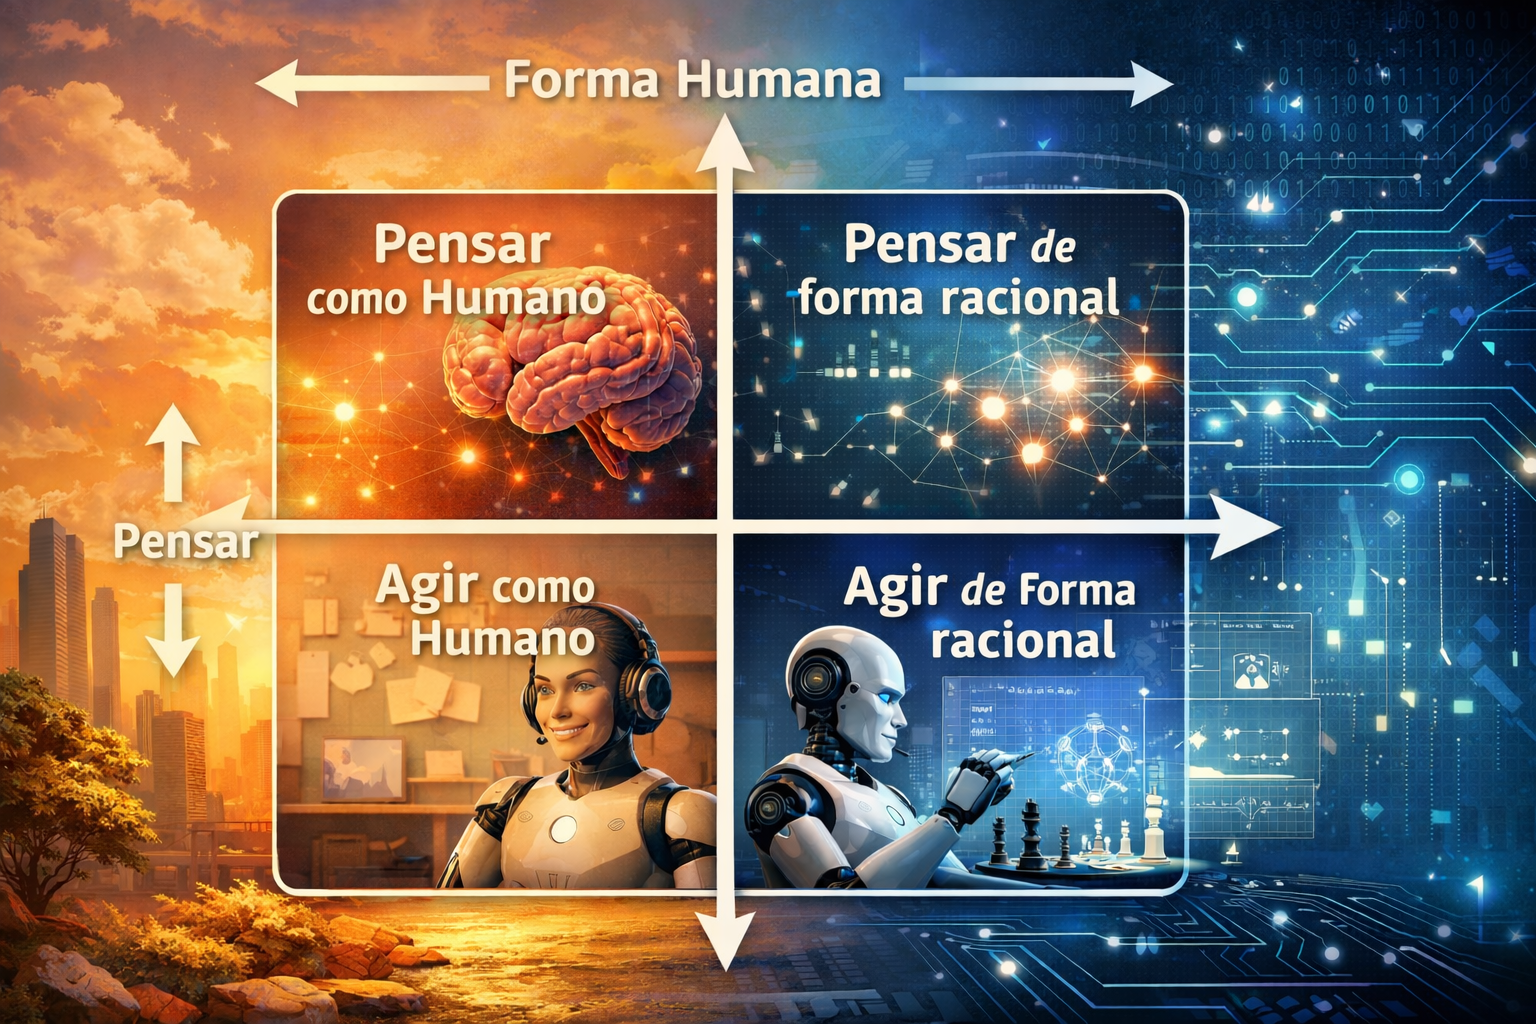
\includegraphics
            [width=0.8\textwidth]{images/pensar-forma.png}
        \end{center}
        
	\end{frame} 

    \begin{frame}{Agir de forma racional}
        \begin{block}{Ideia Geral}
            Essa linha é a definição mais adotada na Computação.        
        \end{block} \pause
		\begin{block}{Poole {\it et al.}, 1998}
			``A Inteligência Computacional é \\o estudo do projeto de agentes inteligentes''
		\end{block}\pause
		\begin{exampleblock}{Exemplo}
			Agentes racionais.
		\end{exampleblock}
	\end{frame}

    \begin{frame}{Agentes Racionais}
        
        \begin{center}
            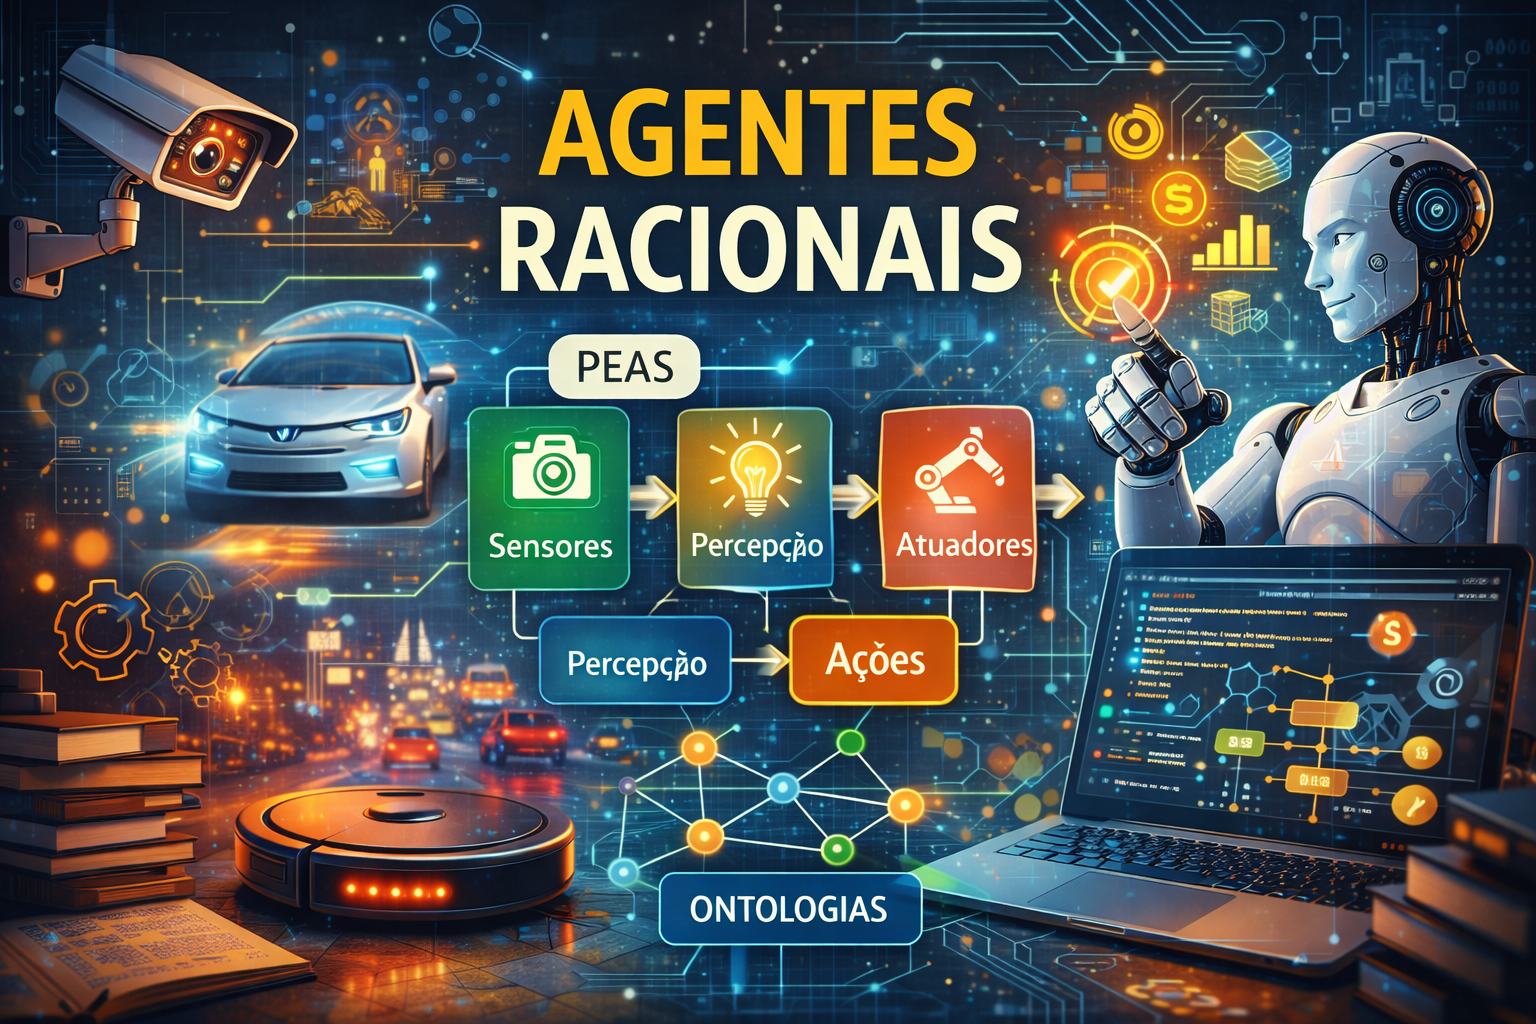
\includegraphics
                [width=\textwidth]{images/agentes-racionais.png}
        \end{center}
        
    \end{frame}

    \begin{frame}{Agir de forma racional}
        \begin{block}{Ideia Geral}
            Essa linha é a definição mais adotada na Computação.        
        \end{block} 
		\begin{block}{Poole {\it et al.}, 1998}
			``A Inteligência Computacional é \\o estudo do projeto de agentes inteligentes''
		\end{block}
		\begin{exampleblock}{Provocação para a Pesquisa em Educação}
			Se um sistema decide o próximo conteúdo para o aluno, \\qual é o papel do professor?
		\end{exampleblock}
	\end{frame}	
	
	\begin{frame}
		\titlepage
	\end{frame}
	
\end{document}